
% This LaTeX was auto-generated from MATLAB code.
% To make changes, update the MATLAB code and republish this document.

\documentclass{article}
\usepackage{graphicx}
\usepackage{color}

\sloppy
\definecolor{lightgray}{gray}{0.5}
\setlength{\parindent}{0pt}

\begin{document}

    
    
\subsection*{Contents}

\begin{itemize}
\setlength{\itemsep}{-1ex}
   \item Define Contour
   \item Define Space
   \item Define Green's function
   \item Integrate
   \item Plot Figure
   \item Transpose All variables for all variables
\end{itemize}
\begin{verbatim}
clear all
% close all;clc

lambda = 633e-9; % Red light wavelength
eps_silver =  -18.295 - 1i*0.48085; % Johnson & Christy,1972 (refractiveindex.info) at 633 nm
load em_constants.mat % Contains varepsilon, mu and c
eps_0 = epsilon_0;
omega = 2*pi*c/lambda; % angular frequency

k_air = 2*pi/lambda; % propagation constant of air
k_silver = omega * sqrt(mu_0*epsilon_0*eps_silver); % propagation constant of silver
\end{verbatim}


\subsection*{Define Contour}

\begin{verbatim}
len = 1e3; % Vector length
kxx = horzcat(linspace(0*k_air,1e-1*k_air,len/2), ...
        linspace(1e-1*k_air,1e1*k_air,len/2),...
        linspace(1e1*k_air,1e3*k_air,len/2));
kxy = horzcat(linspace(-1e4*k_air,-1e-1*k_air,len/2), ...
        linspace(-1e-1*k_air,1e1*k_air,len/2),...
        linspace(1e1*k_air,1e2*k_air,len/2)); % Piece-wise definition for smoother plots


% Find zero location
y_zero = abs(kxy - 0);
y_zero_index = find(y_zero == min(y_zero)); % Index in kxy with the nearest value to 0
c0_x_neg = linspace( -1e4*k_air, 0, len/2);

% Create contour in negative and positive halves separately
% c0_y_neg = kxy(y_zero_index);
c0_y_neg = 0;
c0_x_pos = linspace( 0, 1e4*k_air,  len/2);
% c0_y_pos = kxy(y_zero_index);
c0_y_pos = 0;

C0_neg = [c0_x_neg ; c0_y_neg*ones(1, len/2)];
C0_pos = [c0_x_pos ; c0_y_pos*ones(1, len/2)];
C0 = horzcat(C0_neg, C0_pos);  % Merge the two halves
% C0 = horzcat(C0_pos);
kx = C0(1,:) + 1i*C0(2,:); % make a complex contour along the real axis
\end{verbatim}


\subsection*{Define Space}

\begin{verbatim}
x = linspace(1e-2*lambda,1e4*lambda,2*len/2); % Piece-wise definition for smoother plots
\end{verbatim}


\subsection*{Define Green's function}

\begin{verbatim}
kz_1 = @(kx) sqrt(k_air^2 - kx.^2);
kz_2 = @(kx) sqrt(k_silver^2 - kx.^2);
D = @(kz_1, kz_2) kz_2/eps_silver + kz_1/1;
% G = @(kz_1, kz_2) 1./D;
%
kz_1 = kz_1(kx);
kz_2 = kz_2(kx);
D = D(kz_1, kz_2);
G = 1./D;
dkx = diff(kx);
H = zeros ( 1, length (x));
su = 0;
\end{verbatim}


\subsection*{Integrate}

\begin{verbatim}
for i = 1 : length(x)
    for j = 1 : length(kx) - 1

%         if real(kz_1) > 0
%             kz_1= -real(kz_1) + 1i*imag(kz_1);
%         end
%         if real(kz_2) > 0
%             kz_2 = -real(kz_2) + 1i*imag(kz_2);
%         end
%
% %         Satisfy Imaginary parts
%         if imag(kz_1) > 0
%             kz_1 = conj(kz_1);
%         end
%         if imag(kz_2) > 0
%             kz_2 = conj(kz_2);
%         end
%         if real(kz_1(j)) > 0
%             kz_1(j) = -real(kz_1(j)) + 1i*imag(kz_1(j));
%         end
%         if real(kz_2(j)) > 0
%             kz_2(j) = -real(kz_2(j)) + 1i*imag(kz_2(j));
%         end
%         %
% %         Satisfy Imaginary parts
%         if imag(kz_1(j)) > 0
%             kz_1(j) = conj(kz_1(j));
%         end
%         if imag(kz_2(j)) > 0
%             kz_2(j) = conj(kz_2(j));
%         end
        integrand = G(j)*exp(-1i*kx(j)*x(i));
        su = su + integrand;
    end
    H(i) = su;
    su = 0;
end
\end{verbatim}


\subsection*{Plot Figure}

\begin{par}
loglog(x/lambda, abs(H)/abs(max(H)),'LineWidth',1.4,'Color','black')
\end{par} \vspace{1em}
\begin{verbatim}
loglog(x/lambda, abs(H),'LineWidth',1.4,'Color','black')
set(gcf,'Color','white');

ylabel('$\vert Creeping Wave\vert$',...
'HorizontalAlignment','center',...
    'FontWeight','bold',...
    'FontSize',12,...
    'Interpreter','latex');

% Create xlabel
xlabel('$\frac{x}{\lambda}$',...
    'HorizontalAlignment','center',...
    'FontWeight','bold',...
    'FontSize',12,...
    'Interpreter','latex');

% ylim([10e-10 10e1])
title('Decay Plot of Creeping Wave part');
matlab2tikz('filename',sprintf('nevels_michalski_real_axis_int.tex'))
\end{verbatim}

        \color{lightgray} \begin{verbatim} *** (To disable info messages, pass ['showInfo', false] to matlab2tikz.)
 *** (For all other options, type 'help matlab2tikz'.)
 *** 
 *** 
 *** This is matlab2tikz v1.0.0.
 *** 
 *** The latest updates can be retrieved from
 ***  http://www.mathworks.com/matlabcentral/fileexchange/22022-matlab2tikz-matlab2tikz
 *** where you can also make suggestions and rate matlab2tikz.
 *** For usage instructions, bug reports, the latest development versions and more, see
 ***    https://github.com/matlab2tikz/matlab2tikz,
 ***    https://github.com/matlab2tikz/matlab2tikz/wiki,
 ***    https://github.com/matlab2tikz/matlab2tikz/issues.
 *** 
 *** You will need pgfplots version 1.3 or newer to compile the TikZ output.
\end{verbatim} \color{black}
    
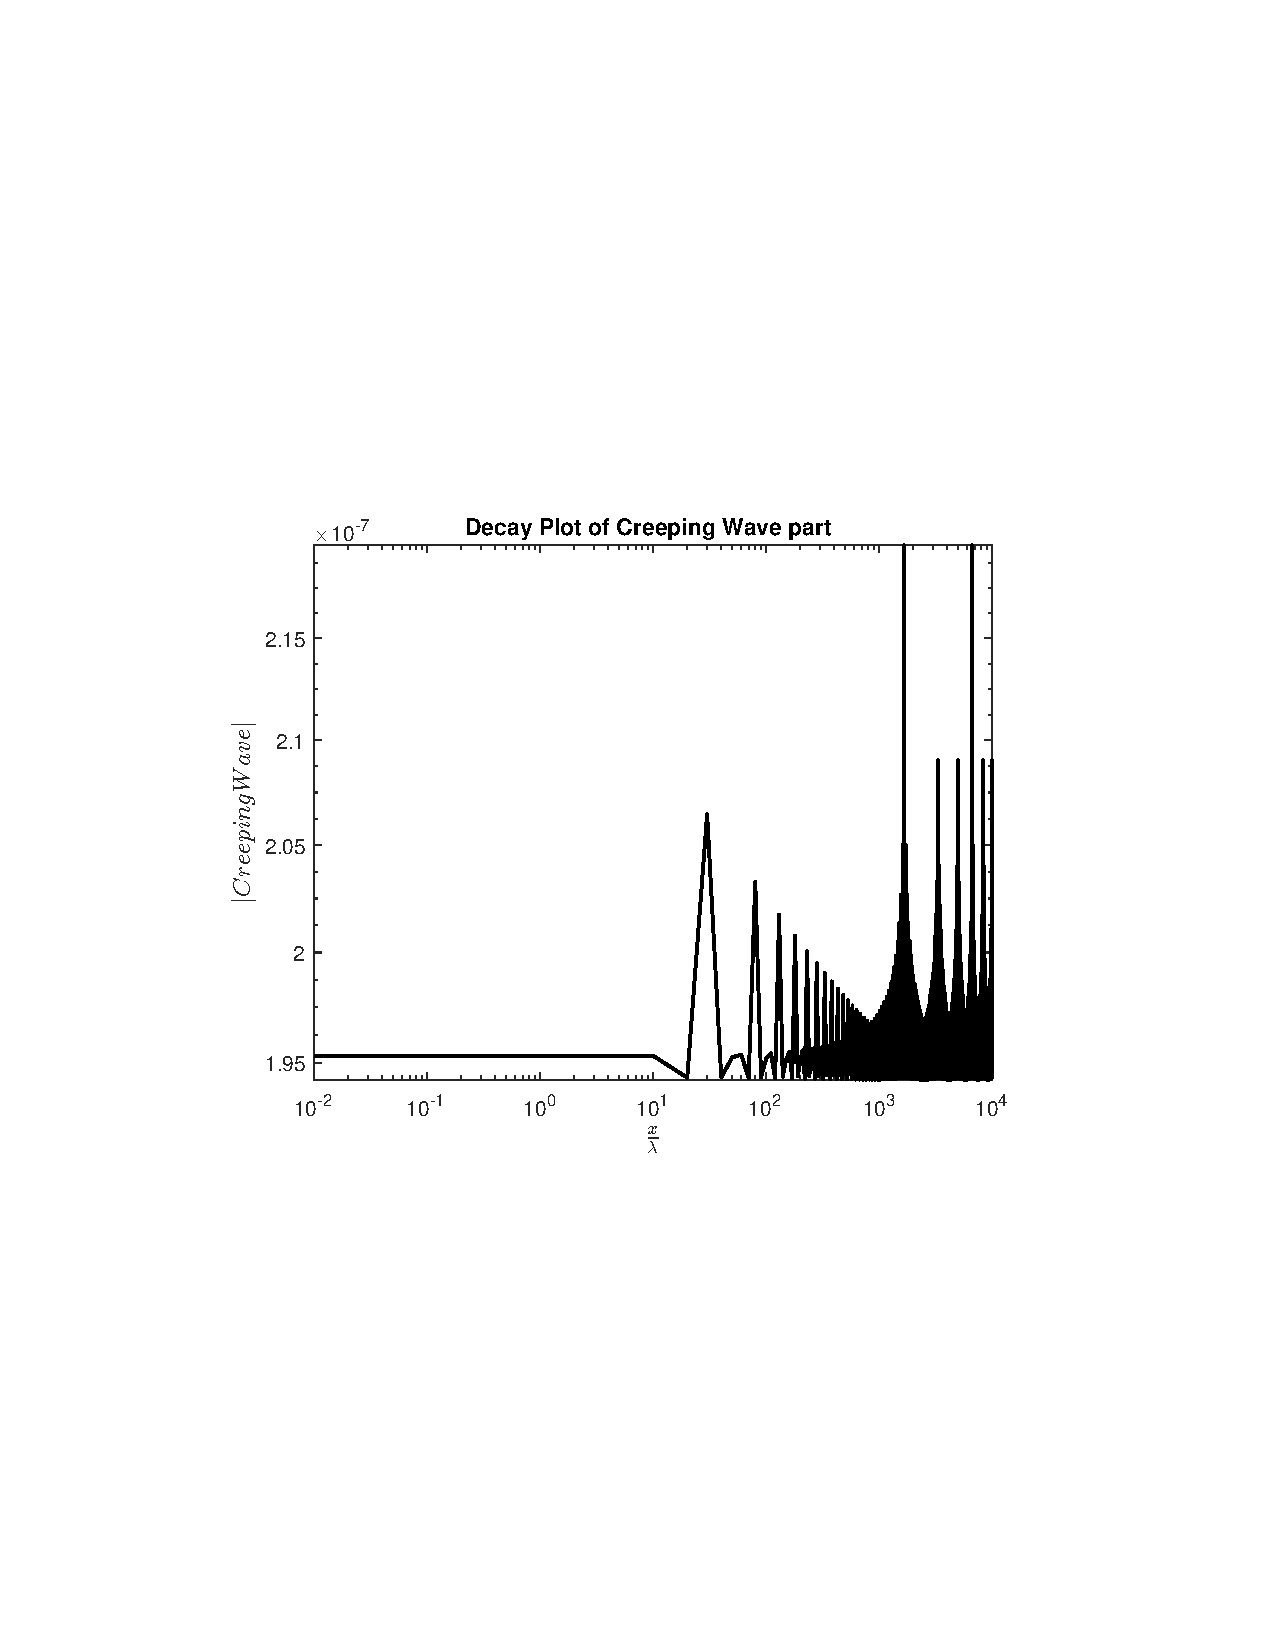
\includegraphics [width=4in]{Nevels_paper_Creeping_wave_part_real_axis_01.pdf}


\subsection*{Transpose All variables for all variables}

\begin{verbatim}
kz_1 = kz_1.';
kz_2 = kz_2.';
D = D.';
G = G.';
H = H.';
kx = kx.';
\end{verbatim}



\end{document}
    
